% Options for packages loaded elsewhere
\PassOptionsToPackage{unicode}{hyperref}
\PassOptionsToPackage{hyphens}{url}
%
\documentclass[
]{article}
\usepackage{lmodern}
\usepackage{amssymb,amsmath}
\usepackage{ifxetex,ifluatex}
\ifnum 0\ifxetex 1\fi\ifluatex 1\fi=0 % if pdftex
  \usepackage[T1]{fontenc}
  \usepackage[utf8]{inputenc}
  \usepackage{textcomp} % provide euro and other symbols
\else % if luatex or xetex
  \usepackage{unicode-math}
  \defaultfontfeatures{Scale=MatchLowercase}
  \defaultfontfeatures[\rmfamily]{Ligatures=TeX,Scale=1}
\fi
% Use upquote if available, for straight quotes in verbatim environments
\IfFileExists{upquote.sty}{\usepackage{upquote}}{}
\IfFileExists{microtype.sty}{% use microtype if available
  \usepackage[]{microtype}
  \UseMicrotypeSet[protrusion]{basicmath} % disable protrusion for tt fonts
}{}
\makeatletter
\@ifundefined{KOMAClassName}{% if non-KOMA class
  \IfFileExists{parskip.sty}{%
    \usepackage{parskip}
  }{% else
    \setlength{\parindent}{0pt}
    \setlength{\parskip}{6pt plus 2pt minus 1pt}}
}{% if KOMA class
  \KOMAoptions{parskip=half}}
\makeatother
\usepackage{xcolor}
\IfFileExists{xurl.sty}{\usepackage{xurl}}{} % add URL line breaks if available
\IfFileExists{bookmark.sty}{\usepackage{bookmark}}{\usepackage{hyperref}}
\hypersetup{
  pdftitle={Blossom Watch 2021},
  pdfauthor={Alan Millington},
  hidelinks,
  pdfcreator={LaTeX via pandoc}}
\urlstyle{same} % disable monospaced font for URLs
\usepackage[margin=1in]{geometry}
\usepackage{longtable,booktabs}
% Correct order of tables after \paragraph or \subparagraph
\usepackage{etoolbox}
\makeatletter
\patchcmd\longtable{\par}{\if@noskipsec\mbox{}\fi\par}{}{}
\makeatother
% Allow footnotes in longtable head/foot
\IfFileExists{footnotehyper.sty}{\usepackage{footnotehyper}}{\usepackage{footnote}}
\makesavenoteenv{longtable}
\usepackage{graphicx,grffile}
\makeatletter
\def\maxwidth{\ifdim\Gin@nat@width>\linewidth\linewidth\else\Gin@nat@width\fi}
\def\maxheight{\ifdim\Gin@nat@height>\textheight\textheight\else\Gin@nat@height\fi}
\makeatother
% Scale images if necessary, so that they will not overflow the page
% margins by default, and it is still possible to overwrite the defaults
% using explicit options in \includegraphics[width, height, ...]{}
\setkeys{Gin}{width=\maxwidth,height=\maxheight,keepaspectratio}
% Set default figure placement to htbp
\makeatletter
\def\fps@figure{htbp}
\makeatother
\setlength{\emergencystretch}{3em} % prevent overfull lines
\providecommand{\tightlist}{%
  \setlength{\itemsep}{0pt}\setlength{\parskip}{0pt}}
\setcounter{secnumdepth}{-\maxdimen} % remove section numbering

\title{Blossom Watch 2021}
\author{Alan Millington}
\date{2021-03-19 16:07:07}

\begin{document}
\maketitle

\begin{longtable}[]{@{}lr@{}}
\toprule
\begin{minipage}[b]{0.41\columnwidth}\raggedright
hashtag\strut
\end{minipage} & \begin{minipage}[b]{0.10\columnwidth}\raggedleft
count\strut
\end{minipage}\tabularnewline
\midrule
\endhead
\begin{minipage}[t]{0.41\columnwidth}\raggedright
blossom\strut
\end{minipage} & \begin{minipage}[t]{0.10\columnwidth}\raggedleft
1174\strut
\end{minipage}\tabularnewline
\begin{minipage}[t]{0.41\columnwidth}\raggedright
blossomwatch\strut
\end{minipage} & \begin{minipage}[t]{0.10\columnwidth}\raggedleft
846\strut
\end{minipage}\tabularnewline
\begin{minipage}[t]{0.41\columnwidth}\raggedright
NationalTrust + BlossomWatch\strut
\end{minipage} & \begin{minipage}[t]{0.10\columnwidth}\raggedleft
19\strut
\end{minipage}\tabularnewline
\begin{minipage}[t]{0.41\columnwidth}\raggedright
EveryoneNeedsNature\strut
\end{minipage} & \begin{minipage}[t]{0.10\columnwidth}\raggedleft
73\strut
\end{minipage}\tabularnewline
\begin{minipage}[t]{0.41\columnwidth}\raggedright
None\strut
\end{minipage} & \begin{minipage}[t]{0.10\columnwidth}\raggedleft
737\strut
\end{minipage}\tabularnewline
\bottomrule
\end{longtable}

\hypertarget{timeline}{%
\section{Timeline}\label{timeline}}

\hypertarget{tweets-by-day}{%
\subsection{Tweets by day}\label{tweets-by-day}}

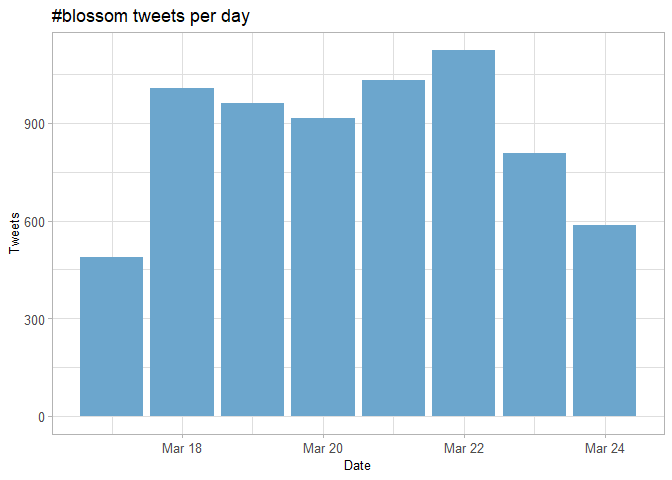
\includegraphics{twitter-blossom-watch-2021_files/figure-latex/tweets-by-day-1.pdf}

\hypertarget{tweets-by-day-and-time}{%
\subsection{Tweets by day and time}\label{tweets-by-day-and-time}}

Filtered for dates March, London time.
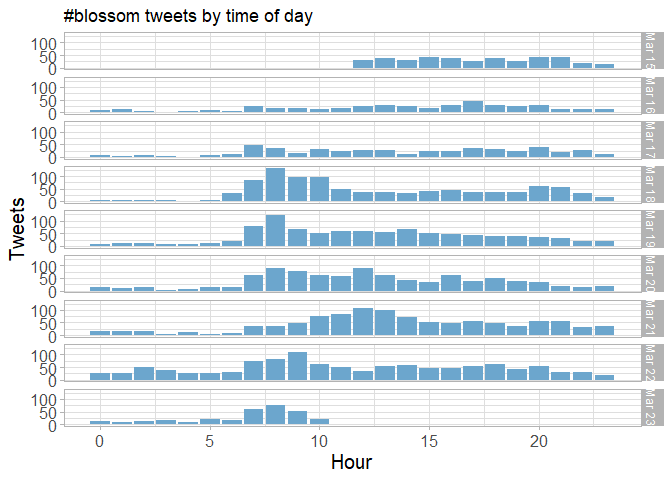
\includegraphics{twitter-blossom-watch-2021_files/figure-latex/tweets-by-day-hour-1.pdf}

\hypertarget{users}{%
\section{Users}\label{users}}

\hypertarget{top-tweeters}{%
\subsection{Top tweeters}\label{top-tweeters}}

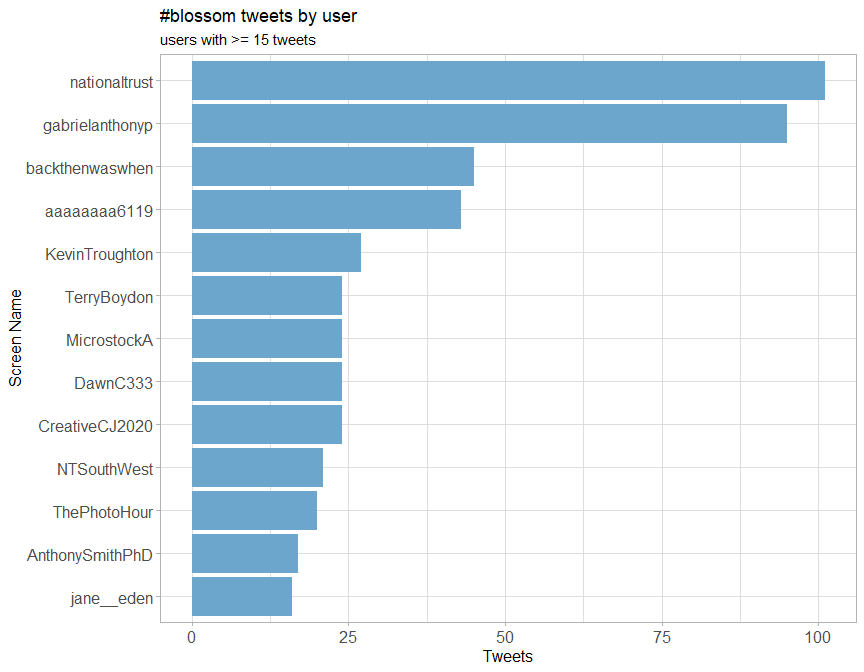
\includegraphics{twitter-blossom-watch-2021_files/figure-latex/tweets-top-users-1.pdf}

\hypertarget{sources}{%
\subsection{Sources}\label{sources}}

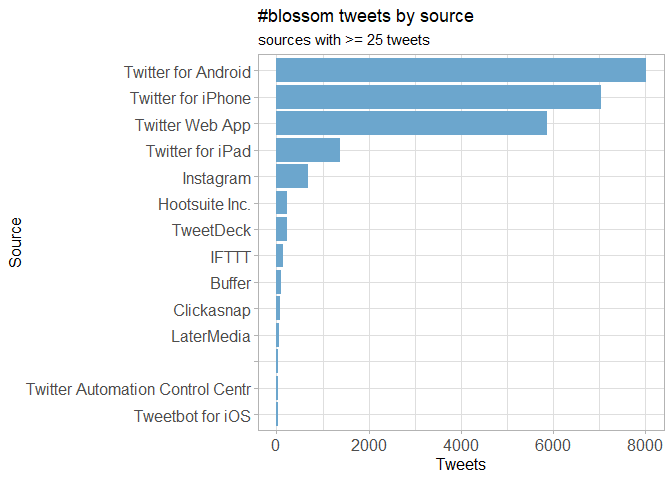
\includegraphics{twitter-blossom-watch-2021_files/figure-latex/tweets-top-sources-1.pdf}

\hypertarget{networks}{%
\section{Networks}\label{networks}}

\hypertarget{replies}{%
\subsection{Replies}\label{replies}}

The ``replies network'', composed from users who reply directly to one
another.

Better to view the original PNG file in the \texttt{data} directory.

\includegraphics{replies_network.png}

\hypertarget{mentions}{%
\subsection{Mentions}\label{mentions}}

The ``mentions network'', where users mention other users in their
tweets.

Better to view the original PNG file in the \texttt{data} directory.

\includegraphics{mentions_network.png}

\hypertarget{retweets}{%
\section{Retweets}\label{retweets}}

\hypertarget{retweet-proportion}{%
\subsection{Retweet proportion}\label{retweet-proportion}}

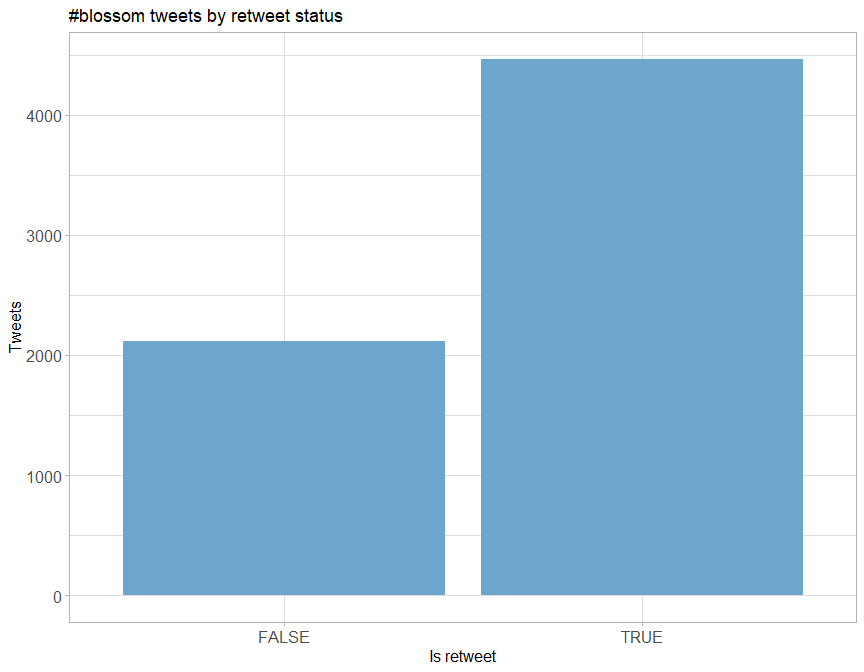
\includegraphics{twitter-blossom-watch-2021_files/figure-latex/is-retweet-1.pdf}

\hypertarget{retweet-count}{%
\subsection{Retweet count}\label{retweet-count}}

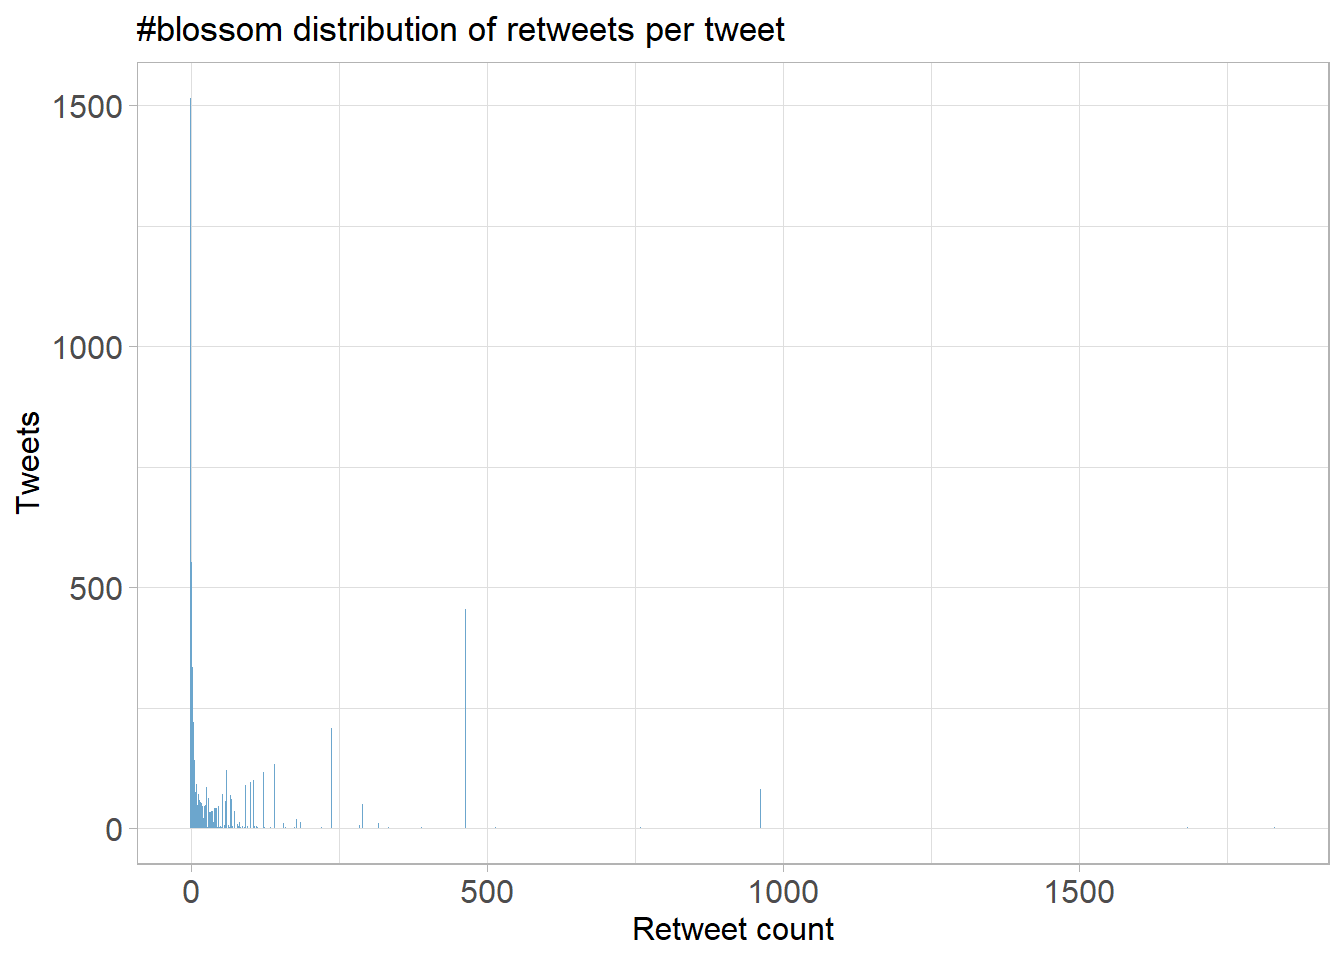
\includegraphics{twitter-blossom-watch-2021_files/figure-latex/retweet-count-1.pdf}

\hypertarget{top-retweets}{%
\subsection{Top retweets}\label{top-retweets}}

\begin{longtable}[]{@{}llr@{}}
\toprule
\begin{minipage}[b]{0.14\columnwidth}\raggedright
screen\_name\strut
\end{minipage} & \begin{minipage}[b]{0.65\columnwidth}\raggedright
text\strut
\end{minipage} & \begin{minipage}[b]{0.12\columnwidth}\raggedleft
retweet\_count\strut
\end{minipage}\tabularnewline
\midrule
\endhead
\begin{minipage}[t]{0.14\columnwidth}\raggedright
KhushnumaKashm1\strut
\end{minipage} & \begin{minipage}[t]{0.65\columnwidth}\raggedright
Apricot \#blossom \#Kashmir \#spring \url{https://t.co/YBDM7JMLbY}\strut
\end{minipage} & \begin{minipage}[t]{0.12\columnwidth}\raggedleft
322\strut
\end{minipage}\tabularnewline
\begin{minipage}[t]{0.14\columnwidth}\raggedright
dadajay001\strut
\end{minipage} & \begin{minipage}[t]{0.65\columnwidth}\raggedright
\textless U+0917\textgreater\textless U+0941\textgreater\textless U+0932\textgreater\textless U+093E\textgreater\textless U+092C\textgreater{}
\textless U+0938\textgreater\textless U+0940\textgreater{}
\textless U+091C\textgreater\textless U+093F\textgreater\textless U+0902\textgreater\textless U+0926\textgreater\textless U+0917\textgreater\textless U+0940\textgreater{}
\textless U+0939\textgreater\textless U+0948\textgreater{}
\textless U+0928\textgreater\textless U+093E\textgreater{}
\textless U+0915\textgreater\textless U+093E\textgreater\textless U+0902\textgreater\textless U+091F\textgreater\textless U+094B\textgreater\textless U+0902\textgreater{}
\textless U+0915\textgreater\textless U+093E\textgreater{}
\textless U+0926\textgreater\textless U+0930\textgreater\textless U+094D\textgreater\textless U+0926\textgreater{}
\textless U+0939\textgreater\textless U+0948\textgreater{}
\textless U+0928\textgreater\textless U+093E\textgreater{}
\textless U+092A\textgreater\textless U+0902\textgreater\textless U+0916\textgreater\textless U+0941\textgreater\textless U+0921\textgreater\textless U+093C\textgreater\textless U+093F\textgreater\textless U+092F\textgreater\textless U+094B\textgreater\textless U+0902\textgreater{}
\textless U+0915\textgreater\textless U+0940\textgreater{}
\textless U+0916\textgreater\textless U+0941\textgreater\textless U+0936\textgreater\textless U+092C\textgreater\textless U+0941\textgreater\ldots.
\textless U+2728\textgreater\textless U+2764\textgreater\textless U+FE0F\textgreater{}
\#Petals \#Blossom \#My\_click \url{https://t.co/kEbXfNpjI7}\strut
\end{minipage} & \begin{minipage}[t]{0.12\columnwidth}\raggedleft
95\strut
\end{minipage}\tabularnewline
\begin{minipage}[t]{0.14\columnwidth}\raggedright
nationaltrust\strut
\end{minipage} & \begin{minipage}[t]{0.65\columnwidth}\raggedright
Everywhere these delicate flowers emerge, they bring delight with them.
Thanks to everyone who's helped spread the joys of blossom so far - keep
the photos coming with \#BlossomWatch. Photos: Joanna A, Catherine A,
Shonali B, Cara W. \url{https://t.co/6znNDEdvKC}\strut
\end{minipage} & \begin{minipage}[t]{0.12\columnwidth}\raggedleft
87\strut
\end{minipage}\tabularnewline
\begin{minipage}[t]{0.14\columnwidth}\raggedright
nationaltrust\strut
\end{minipage} & \begin{minipage}[t]{0.65\columnwidth}\raggedright
\textless U+0001F338\textgreater\#BlossomWatch\textless U+0001F338\textgreater{}
Lockdowns have changed the nation's relationship with nature for the
better. We are feeling more connected thanks to our daily strolls and
taking more notice of the changing seasons.
\url{https://t.co/JtIkqgUorV}\strut
\end{minipage} & \begin{minipage}[t]{0.12\columnwidth}\raggedleft
78\strut
\end{minipage}\tabularnewline
\begin{minipage}[t]{0.14\columnwidth}\raggedright
ampomata\strut
\end{minipage} & \begin{minipage}[t]{0.65\columnwidth}\raggedright
This is my new painting ``Bed Of Roses''. You can check it out here:
\url{https://t.co/GoYnqeM1YY} \#art \#arte \#oleo \#kunst \#oilpainting
\#contemporaryart \#ArtistOnTwitter \#blossom \#flower \#floral \#spring
\#pink \#red \#roses \#field \#artprints \#flowers \#garden
\url{https://t.co/7y9skbUaMs}\strut
\end{minipage} & \begin{minipage}[t]{0.12\columnwidth}\raggedleft
67\strut
\end{minipage}\tabularnewline
\begin{minipage}[t]{0.14\columnwidth}\raggedright
MikeDoylePhotos\strut
\end{minipage} & \begin{minipage}[t]{0.65\columnwidth}\raggedright
Spring colour at Sheffield Park, East Sussex. \#Sussex \#England
\#NationalTrust \#landscape \#landscapephotography \#travel
\#travelphotography \#photo \#photography \#photooftheday
\#NaturePhotography \url{https://t.co/uFdcfnor39}\strut
\end{minipage} & \begin{minipage}[t]{0.12\columnwidth}\raggedleft
51\strut
\end{minipage}\tabularnewline
\begin{minipage}[t]{0.14\columnwidth}\raggedright
nationaltrust\strut
\end{minipage} & \begin{minipage}[t]{0.65\columnwidth}\raggedright
\textless U+0001F338\textgreater{} With buds beginning to burst we’re
asking you to help us track the blossom as it appears. Just add
\#BlossomWatch to your tweets, with location settings on, to add your
sightings to our map: \url{https://t.co/Oto3d8C9ZQ}
\url{https://t.co/9a3Q2umF03}\strut
\end{minipage} & \begin{minipage}[t]{0.12\columnwidth}\raggedleft
49\strut
\end{minipage}\tabularnewline
\begin{minipage}[t]{0.14\columnwidth}\raggedright
nationaltrust\strut
\end{minipage} & \begin{minipage}[t]{0.65\columnwidth}\raggedright
As the days lengthen, take an early evening walk and listen out for the
blackbird chorus. Perched as high as they can, they fill the spring air
with song. \#EveryoneNeedsNature \url{https://t.co/fokl4eudbL}\strut
\end{minipage} & \begin{minipage}[t]{0.12\columnwidth}\raggedleft
42\strut
\end{minipage}\tabularnewline
\begin{minipage}[t]{0.14\columnwidth}\raggedright
nationaltrust\strut
\end{minipage} & \begin{minipage}[t]{0.65\columnwidth}\raggedright
This spring, spend time under the delicate blooms of a blossom tree and
watch as nature's confetti dances to the ground. Share your pictures of
pink, white and green with us using
\#BlossomWatch\textless U+0001F338\textgreater{}
\url{https://t.co/0WFkQ61nfD}\strut
\end{minipage} & \begin{minipage}[t]{0.12\columnwidth}\raggedleft
40\strut
\end{minipage}\tabularnewline
\begin{minipage}[t]{0.14\columnwidth}\raggedright
nationaltrust\strut
\end{minipage} & \begin{minipage}[t]{0.65\columnwidth}\raggedright
A bright burst of yellow Forsythia is like the sunshine after the rain.
Flowering with the spring bulbs, these blooms are a sure sign of the
gardens we care for reawakening after winter. \#EveryoneNeedsNature
\url{https://t.co/eRc7pCw2nJ}\strut
\end{minipage} & \begin{minipage}[t]{0.12\columnwidth}\raggedleft
39\strut
\end{minipage}\tabularnewline
\bottomrule
\end{longtable}

\hypertarget{favourites}{%
\section{Favourites}\label{favourites}}

\hypertarget{favourite-proportion}{%
\subsection{Favourite proportion}\label{favourite-proportion}}

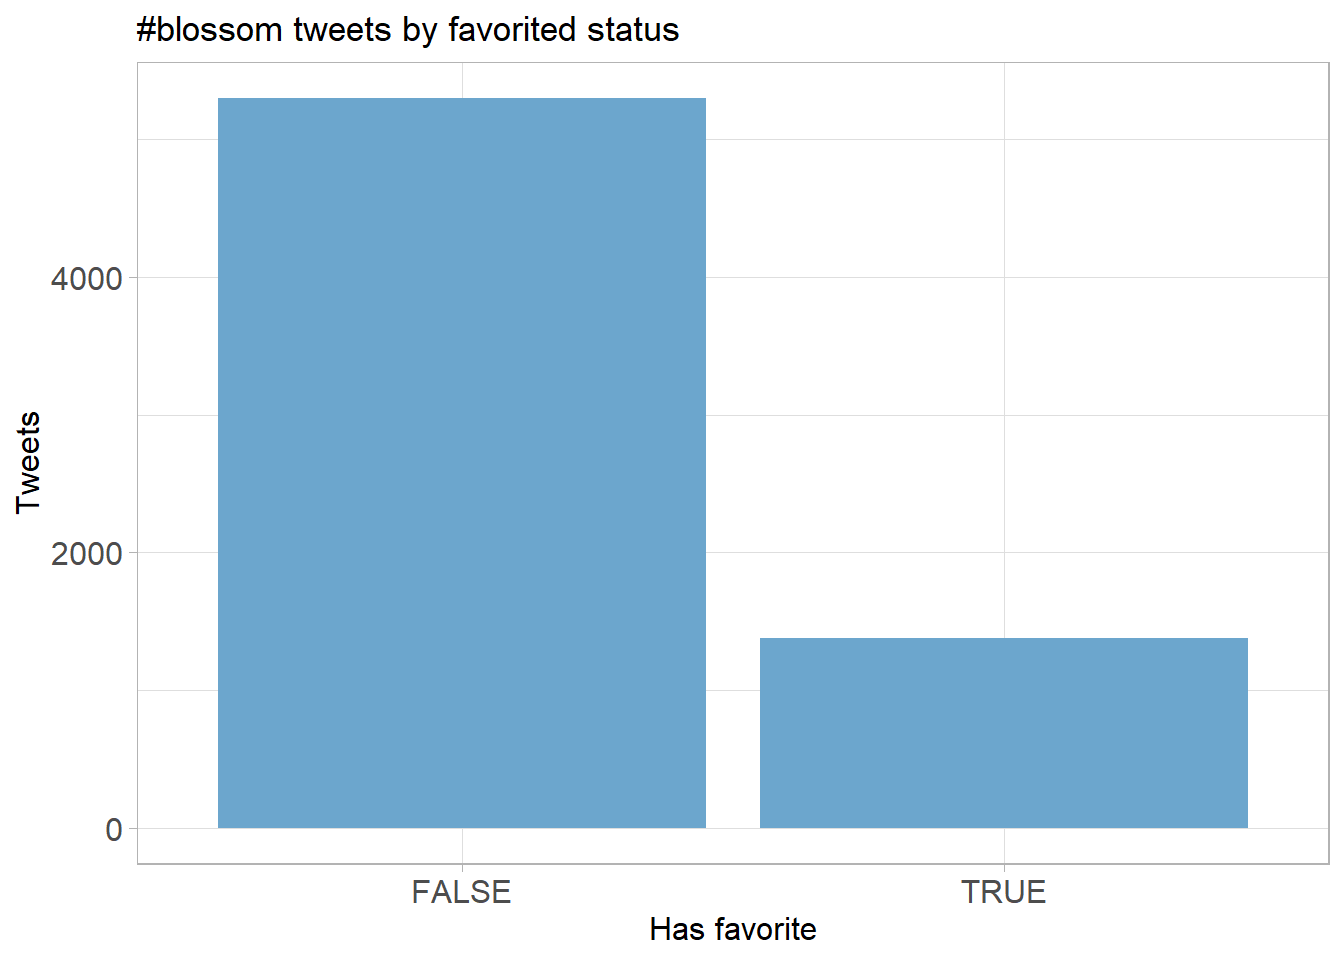
\includegraphics{twitter-blossom-watch-2021_files/figure-latex/has-favorite-1.pdf}

\hypertarget{favourite-count}{%
\subsection{Favourite count}\label{favourite-count}}

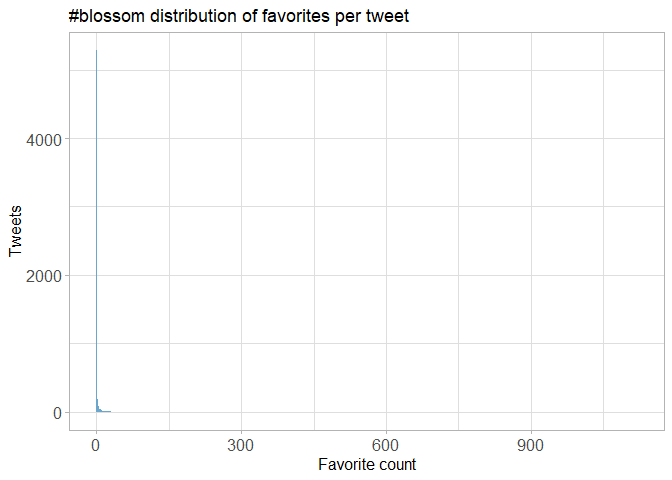
\includegraphics{twitter-blossom-watch-2021_files/figure-latex/favorite-count-1.pdf}

\hypertarget{top-favourites}{%
\subsection{Top favourites}\label{top-favourites}}

\begin{longtable}[]{@{}llr@{}}
\toprule
\begin{minipage}[b]{0.22\columnwidth}\raggedright
screen\_name\strut
\end{minipage} & \begin{minipage}[b]{0.49\columnwidth}\raggedright
text\strut
\end{minipage} & \begin{minipage}[b]{0.21\columnwidth}\raggedleft
favorite\_count\strut
\end{minipage}\tabularnewline
\midrule
\endhead
\begin{minipage}[t]{0.22\columnwidth}\raggedright
nationaltrust\strut
\end{minipage} & \begin{minipage}[t]{0.49\columnwidth}\raggedright
\textless U+0001F338\textgreater\#BlossomWatch\textless U+0001F338\textgreater{}
Lockdowns have changed the nation's relationship with nature for the
better. We are feeling more connected thanks to our daily strolls and
taking more notice of the changing seasons.
\url{https://t.co/JtIkqgUorV}\strut
\end{minipage} & \begin{minipage}[t]{0.21\columnwidth}\raggedleft
512\strut
\end{minipage}\tabularnewline
\begin{minipage}[t]{0.22\columnwidth}\raggedright
nationaltrust\strut
\end{minipage} & \begin{minipage}[t]{0.49\columnwidth}\raggedright
Everywhere these delicate flowers emerge, they bring delight with them.
Thanks to everyone who's helped spread the joys of blossom so far - keep
the photos coming with \#BlossomWatch. Photos: Joanna A, Catherine A,
Shonali B, Cara W. \url{https://t.co/6znNDEdvKC}\strut
\end{minipage} & \begin{minipage}[t]{0.21\columnwidth}\raggedleft
509\strut
\end{minipage}\tabularnewline
\begin{minipage}[t]{0.22\columnwidth}\raggedright
nationaltrust\strut
\end{minipage} & \begin{minipage}[t]{0.49\columnwidth}\raggedright
Nature's alarm clock is getting louder with each new day as the birds
look to find their spring mates. Which birds are waking you up in the
morning? Photos: Jenni B, @NTCastleWard \#EveryoneNeedsNature
\url{https://t.co/qFLlRf3gL7}\strut
\end{minipage} & \begin{minipage}[t]{0.21\columnwidth}\raggedleft
412\strut
\end{minipage}\tabularnewline
\begin{minipage}[t]{0.22\columnwidth}\raggedright
MikeDoylePhotos\strut
\end{minipage} & \begin{minipage}[t]{0.49\columnwidth}\raggedright
Spring colour at Sheffield Park, East Sussex. \#Sussex \#England
\#NationalTrust \#landscape \#landscapephotography \#travel
\#travelphotography \#photo \#photography \#photooftheday
\#NaturePhotography \url{https://t.co/uFdcfnor39}\strut
\end{minipage} & \begin{minipage}[t]{0.21\columnwidth}\raggedleft
368\strut
\end{minipage}\tabularnewline
\begin{minipage}[t]{0.22\columnwidth}\raggedright
nationaltrust\strut
\end{minipage} & \begin{minipage}[t]{0.49\columnwidth}\raggedright
As the days lengthen, take an early evening walk and listen out for the
blackbird chorus. Perched as high as they can, they fill the spring air
with song. \#EveryoneNeedsNature \url{https://t.co/fokl4eudbL}\strut
\end{minipage} & \begin{minipage}[t]{0.21\columnwidth}\raggedleft
366\strut
\end{minipage}\tabularnewline
\begin{minipage}[t]{0.22\columnwidth}\raggedright
KhushnumaKashm1\strut
\end{minipage} & \begin{minipage}[t]{0.49\columnwidth}\raggedright
Apricot \#blossom \#Kashmir \#spring \url{https://t.co/YBDM7JMLbY}\strut
\end{minipage} & \begin{minipage}[t]{0.21\columnwidth}\raggedleft
348\strut
\end{minipage}\tabularnewline
\begin{minipage}[t]{0.22\columnwidth}\raggedright
nationaltrust\strut
\end{minipage} & \begin{minipage}[t]{0.49\columnwidth}\raggedright
A bright burst of yellow Forsythia is like the sunshine after the rain.
Flowering with the spring bulbs, these blooms are a sure sign of the
gardens we care for reawakening after winter. \#EveryoneNeedsNature
\url{https://t.co/eRc7pCw2nJ}\strut
\end{minipage} & \begin{minipage}[t]{0.21\columnwidth}\raggedleft
318\strut
\end{minipage}\tabularnewline
\begin{minipage}[t]{0.22\columnwidth}\raggedright
nationaltrust\strut
\end{minipage} & \begin{minipage}[t]{0.49\columnwidth}\raggedright
This spring, spend time under the delicate blooms of a blossom tree and
watch as nature's confetti dances to the ground. Share your pictures of
pink, white and green with us using
\#BlossomWatch\textless U+0001F338\textgreater{}
\url{https://t.co/0WFkQ61nfD}\strut
\end{minipage} & \begin{minipage}[t]{0.21\columnwidth}\raggedleft
278\strut
\end{minipage}\tabularnewline
\begin{minipage}[t]{0.22\columnwidth}\raggedright
MikeDoylePhotos\strut
\end{minipage} & \begin{minipage}[t]{0.49\columnwidth}\raggedright
Some more spring colour at Sheffield Park, East Sussex. \#Sussex
\#England \#NationalTrust \#landscape \#landscapephotography \#travel
\#travelphotography \#photo \#photography \#photooftheday
\#NaturePhotography \url{https://t.co/N5aG6i4wW5}\strut
\end{minipage} & \begin{minipage}[t]{0.21\columnwidth}\raggedleft
228\strut
\end{minipage}\tabularnewline
\begin{minipage}[t]{0.22\columnwidth}\raggedright
nationaltrust\strut
\end{minipage} & \begin{minipage}[t]{0.49\columnwidth}\raggedright
\textless U+0001F338\textgreater{} With buds beginning to burst we’re
asking you to help us track the blossom as it appears. Just add
\#BlossomWatch to your tweets, with location settings on, to add your
sightings to our map: \url{https://t.co/Oto3d8C9ZQ}
\url{https://t.co/9a3Q2umF03}\strut
\end{minipage} & \begin{minipage}[t]{0.21\columnwidth}\raggedleft
210\strut
\end{minipage}\tabularnewline
\bottomrule
\end{longtable}

\hypertarget{quotes}{%
\section{Quotes}\label{quotes}}

\hypertarget{quote-proportion}{%
\subsection{Quote proportion}\label{quote-proportion}}

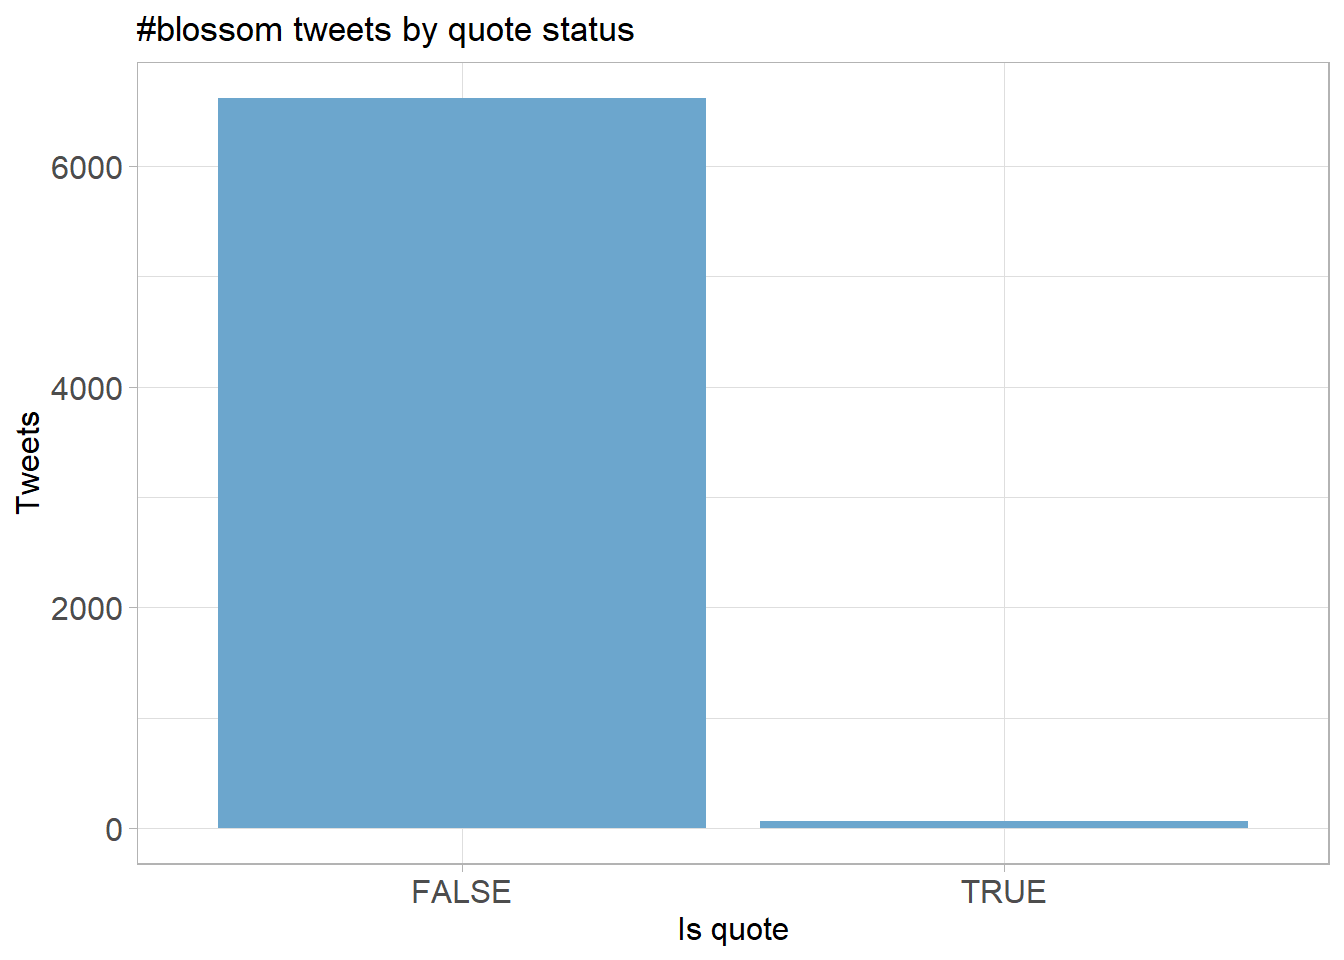
\includegraphics{twitter-blossom-watch-2021_files/figure-latex/is-quote-1.pdf}

\hypertarget{quote-count}{%
\subsection{Quote count}\label{quote-count}}

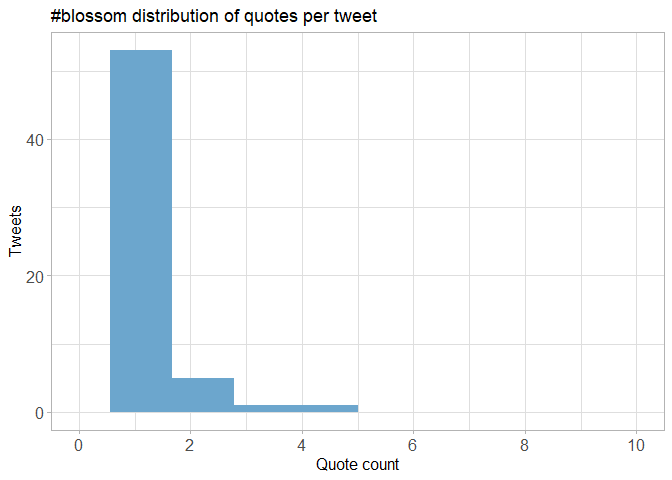
\includegraphics{twitter-blossom-watch-2021_files/figure-latex/quotes-count-1.pdf}

\hypertarget{top-quotes}{%
\subsection{Top quotes}\label{top-quotes}}

Joining, by = ``quoted\_status\_id''

\begin{longtable}[]{@{}llr@{}}
\toprule
\begin{minipage}[b]{0.23\columnwidth}\raggedright
screen\_name\strut
\end{minipage} & \begin{minipage}[b]{0.42\columnwidth}\raggedright
text\strut
\end{minipage} & \begin{minipage}[b]{0.18\columnwidth}\raggedleft
quote\_count\strut
\end{minipage}\tabularnewline
\midrule
\endhead
\begin{minipage}[t]{0.23\columnwidth}\raggedright
WadesWords13\strut
\end{minipage} & \begin{minipage}[t]{0.42\columnwidth}\raggedright
\#BlossomWatch \#BuryStEdmunds \#Suffolk
\textless U+0001F600\textgreater{} \url{https://t.co/3K9z3736Qa}
\url{https://t.co/1vHuj2wDlX}\strut
\end{minipage} & \begin{minipage}[t]{0.18\columnwidth}\raggedleft
3\strut
\end{minipage}\tabularnewline
\begin{minipage}[t]{0.23\columnwidth}\raggedright
wearealtervego\strut
\end{minipage} & \begin{minipage}[t]{0.42\columnwidth}\raggedright
Taking in the \#nature around us\ldots\#andbreathe \#blossomwatch
\#savethebees \#savetheworld \url{https://t.co/9OKBi1ot9E}\strut
\end{minipage} & \begin{minipage}[t]{0.18\columnwidth}\raggedleft
3\strut
\end{minipage}\tabularnewline
\begin{minipage}[t]{0.23\columnwidth}\raggedright
GillianFoxcroft\strut
\end{minipage} & \begin{minipage}[t]{0.42\columnwidth}\raggedright
Wonderful initiative by @nationaltrust Lucky enough to live near
@KedlestonNT where this blackthorn was heralding spring, but blossom is
accessible in our towns and cities too \#BlossomWatch
\url{https://t.co/l3nMn9dvGe} \url{https://t.co/Nri4nxd3vL}\strut
\end{minipage} & \begin{minipage}[t]{0.18\columnwidth}\raggedleft
3\strut
\end{minipage}\tabularnewline
\begin{minipage}[t]{0.23\columnwidth}\raggedright
DerbyUniPress\strut
\end{minipage} & \begin{minipage}[t]{0.42\columnwidth}\raggedright
Research @DerbyUni is making important contributions to initiatives
designed to enhance our \#wellbeing and strengthen our relationship with
\#nature, such as @nationaltrust \#BlossomWatch, which has been launched
today. @findingnature \url{https://t.co/c4ZAhGJs1Q}\strut
\end{minipage} & \begin{minipage}[t]{0.18\columnwidth}\raggedleft
3\strut
\end{minipage}\tabularnewline
\begin{minipage}[t]{0.23\columnwidth}\raggedright
JonathanD1962\strut
\end{minipage} & \begin{minipage}[t]{0.42\columnwidth}\raggedright
@issybryonyh \#BlossomWatch \url{https://t.co/9CLkjUkytC}\strut
\end{minipage} & \begin{minipage}[t]{0.18\columnwidth}\raggedleft
3\strut
\end{minipage}\tabularnewline
\begin{minipage}[t]{0.23\columnwidth}\raggedright
MiriamDobson\strut
\end{minipage} & \begin{minipage}[t]{0.42\columnwidth}\raggedright
Great blog \& paper! \#BlossomWatch is such a fantastic opportunity to
engage with moments in nature - these simple moments of noticing are so
important for wellbeing (as this research demonstrates!)
\url{https://t.co/pBwUoaQ3ZS}\strut
\end{minipage} & \begin{minipage}[t]{0.18\columnwidth}\raggedleft
3\strut
\end{minipage}\tabularnewline
\begin{minipage}[t]{0.23\columnwidth}\raggedright
weather2travel\strut
\end{minipage} & \begin{minipage}[t]{0.42\columnwidth}\raggedright
Will you be joining @nationaltrust \#BlossomWatch?
\textless U+0001F338\textgreater\textless U+0001F440\textgreater{}
\#thursdaymorning \#ThoughtForTheDay \#spring \#bliss
\url{https://t.co/aiQYIY1n5N}\strut
\end{minipage} & \begin{minipage}[t]{0.18\columnwidth}\raggedleft
2\strut
\end{minipage}\tabularnewline
\begin{minipage}[t]{0.23\columnwidth}\raggedright
HeiniHeikkil\strut
\end{minipage} & \begin{minipage}[t]{0.42\columnwidth}\raggedright
Mesmerising, refreshing blossom shared by millions in social media
\textless U+0001F338\textgreater\#UKhanami \#BlossomWatch
\url{https://t.co/Ut9p5H0aEL}\strut
\end{minipage} & \begin{minipage}[t]{0.18\columnwidth}\raggedleft
2\strut
\end{minipage}\tabularnewline
\begin{minipage}[t]{0.23\columnwidth}\raggedright
NaturalEngland\strut
\end{minipage} & \begin{minipage}[t]{0.42\columnwidth}\raggedright
Our research shows that nature is more important than ever to us since
the pandemic started. We're taking more notice of small changes in
nature and signs of spring, like beautiful apple blossom. Share your
pictures of blossom with @NationalTrust using
\textless U+0001F338\textgreater\#BlossomWatch
\textless U+0001F338\textgreater{} \url{https://t.co/KlDTIYa46E}\strut
\end{minipage} & \begin{minipage}[t]{0.18\columnwidth}\raggedleft
2\strut
\end{minipage}\tabularnewline
\begin{minipage}[t]{0.23\columnwidth}\raggedright
radiowinch\strut
\end{minipage} & \begin{minipage}[t]{0.42\columnwidth}\raggedright
Spring is on the way. Celebrate the arrival of blossom near you with
\#BlossomWatch share your photos \url{https://t.co/B0TuHmf6Sk}\strut
\end{minipage} & \begin{minipage}[t]{0.18\columnwidth}\raggedleft
2\strut
\end{minipage}\tabularnewline
\bottomrule
\end{longtable}

\hypertarget{media}{%
\section{Media}\label{media}}

\hypertarget{media-count}{%
\subsection{Media count}\label{media-count}}

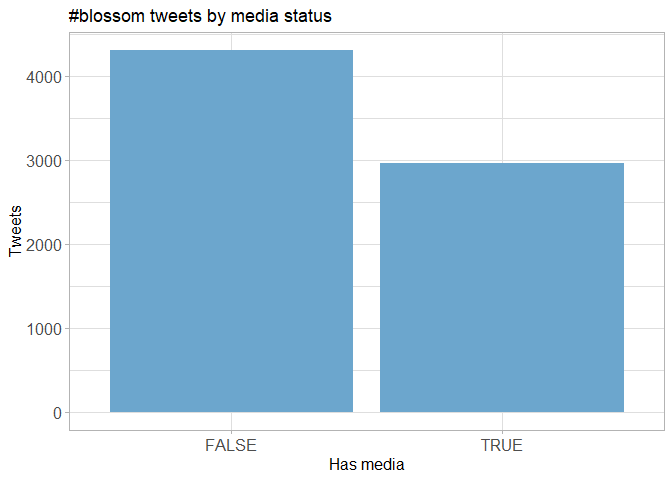
\includegraphics{twitter-blossom-watch-2021_files/figure-latex/has-media-1.pdf}

\hypertarget{top-media}{%
\subsection{Top media}\label{top-media}}

\begin{longtable}[]{@{}llr@{}}
\toprule
\begin{minipage}[b]{0.22\columnwidth}\raggedright
screen\_name\strut
\end{minipage} & \begin{minipage}[b]{0.49\columnwidth}\raggedright
text\strut
\end{minipage} & \begin{minipage}[b]{0.21\columnwidth}\raggedleft
favorite\_count\strut
\end{minipage}\tabularnewline
\midrule
\endhead
\begin{minipage}[t]{0.22\columnwidth}\raggedright
nationaltrust\strut
\end{minipage} & \begin{minipage}[t]{0.49\columnwidth}\raggedright
\textless U+0001F338\textgreater\#BlossomWatch\textless U+0001F338\textgreater{}
Lockdowns have changed the nation's relationship with nature for the
better. We are feeling more connected thanks to our daily strolls and
taking more notice of the changing seasons.
\url{https://t.co/JtIkqgUorV}\strut
\end{minipage} & \begin{minipage}[t]{0.21\columnwidth}\raggedleft
512\strut
\end{minipage}\tabularnewline
\begin{minipage}[t]{0.22\columnwidth}\raggedright
nationaltrust\strut
\end{minipage} & \begin{minipage}[t]{0.49\columnwidth}\raggedright
Everywhere these delicate flowers emerge, they bring delight with them.
Thanks to everyone who's helped spread the joys of blossom so far - keep
the photos coming with \#BlossomWatch. Photos: Joanna A, Catherine A,
Shonali B, Cara W. \url{https://t.co/6znNDEdvKC}\strut
\end{minipage} & \begin{minipage}[t]{0.21\columnwidth}\raggedleft
509\strut
\end{minipage}\tabularnewline
\begin{minipage}[t]{0.22\columnwidth}\raggedright
nationaltrust\strut
\end{minipage} & \begin{minipage}[t]{0.49\columnwidth}\raggedright
Nature's alarm clock is getting louder with each new day as the birds
look to find their spring mates. Which birds are waking you up in the
morning? Photos: Jenni B, @NTCastleWard \#EveryoneNeedsNature
\url{https://t.co/qFLlRf3gL7}\strut
\end{minipage} & \begin{minipage}[t]{0.21\columnwidth}\raggedleft
412\strut
\end{minipage}\tabularnewline
\begin{minipage}[t]{0.22\columnwidth}\raggedright
MikeDoylePhotos\strut
\end{minipage} & \begin{minipage}[t]{0.49\columnwidth}\raggedright
Spring colour at Sheffield Park, East Sussex. \#Sussex \#England
\#NationalTrust \#landscape \#landscapephotography \#travel
\#travelphotography \#photo \#photography \#photooftheday
\#NaturePhotography \url{https://t.co/uFdcfnor39}\strut
\end{minipage} & \begin{minipage}[t]{0.21\columnwidth}\raggedleft
368\strut
\end{minipage}\tabularnewline
\begin{minipage}[t]{0.22\columnwidth}\raggedright
nationaltrust\strut
\end{minipage} & \begin{minipage}[t]{0.49\columnwidth}\raggedright
As the days lengthen, take an early evening walk and listen out for the
blackbird chorus. Perched as high as they can, they fill the spring air
with song. \#EveryoneNeedsNature \url{https://t.co/fokl4eudbL}\strut
\end{minipage} & \begin{minipage}[t]{0.21\columnwidth}\raggedleft
366\strut
\end{minipage}\tabularnewline
\begin{minipage}[t]{0.22\columnwidth}\raggedright
KhushnumaKashm1\strut
\end{minipage} & \begin{minipage}[t]{0.49\columnwidth}\raggedright
Apricot \#blossom \#Kashmir \#spring \url{https://t.co/YBDM7JMLbY}\strut
\end{minipage} & \begin{minipage}[t]{0.21\columnwidth}\raggedleft
348\strut
\end{minipage}\tabularnewline
\begin{minipage}[t]{0.22\columnwidth}\raggedright
nationaltrust\strut
\end{minipage} & \begin{minipage}[t]{0.49\columnwidth}\raggedright
A bright burst of yellow Forsythia is like the sunshine after the rain.
Flowering with the spring bulbs, these blooms are a sure sign of the
gardens we care for reawakening after winter. \#EveryoneNeedsNature
\url{https://t.co/eRc7pCw2nJ}\strut
\end{minipage} & \begin{minipage}[t]{0.21\columnwidth}\raggedleft
318\strut
\end{minipage}\tabularnewline
\begin{minipage}[t]{0.22\columnwidth}\raggedright
nationaltrust\strut
\end{minipage} & \begin{minipage}[t]{0.49\columnwidth}\raggedright
This spring, spend time under the delicate blooms of a blossom tree and
watch as nature's confetti dances to the ground. Share your pictures of
pink, white and green with us using
\#BlossomWatch\textless U+0001F338\textgreater{}
\url{https://t.co/0WFkQ61nfD}\strut
\end{minipage} & \begin{minipage}[t]{0.21\columnwidth}\raggedleft
278\strut
\end{minipage}\tabularnewline
\begin{minipage}[t]{0.22\columnwidth}\raggedright
MikeDoylePhotos\strut
\end{minipage} & \begin{minipage}[t]{0.49\columnwidth}\raggedright
Some more spring colour at Sheffield Park, East Sussex. \#Sussex
\#England \#NationalTrust \#landscape \#landscapephotography \#travel
\#travelphotography \#photo \#photography \#photooftheday
\#NaturePhotography \url{https://t.co/N5aG6i4wW5}\strut
\end{minipage} & \begin{minipage}[t]{0.21\columnwidth}\raggedleft
228\strut
\end{minipage}\tabularnewline
\begin{minipage}[t]{0.22\columnwidth}\raggedright
nationaltrust\strut
\end{minipage} & \begin{minipage}[t]{0.49\columnwidth}\raggedright
\textless U+0001F338\textgreater{} With buds beginning to burst we’re
asking you to help us track the blossom as it appears. Just add
\#BlossomWatch to your tweets, with location settings on, to add your
sightings to our map: \url{https://t.co/Oto3d8C9ZQ}
\url{https://t.co/9a3Q2umF03}\strut
\end{minipage} & \begin{minipage}[t]{0.21\columnwidth}\raggedleft
210\strut
\end{minipage}\tabularnewline
\bottomrule
\end{longtable}

\hypertarget{most-liked-media-image}{%
\subsubsection{Most liked media image}\label{most-liked-media-image}}

\includegraphics{list("http://pbs.twimg.com/media/Ewv2n0OXMAAyWfP.jpg")}

\hypertarget{tweet-text}{%
\section{Tweet text}\label{tweet-text}}

The 100 words used 3 or more times.

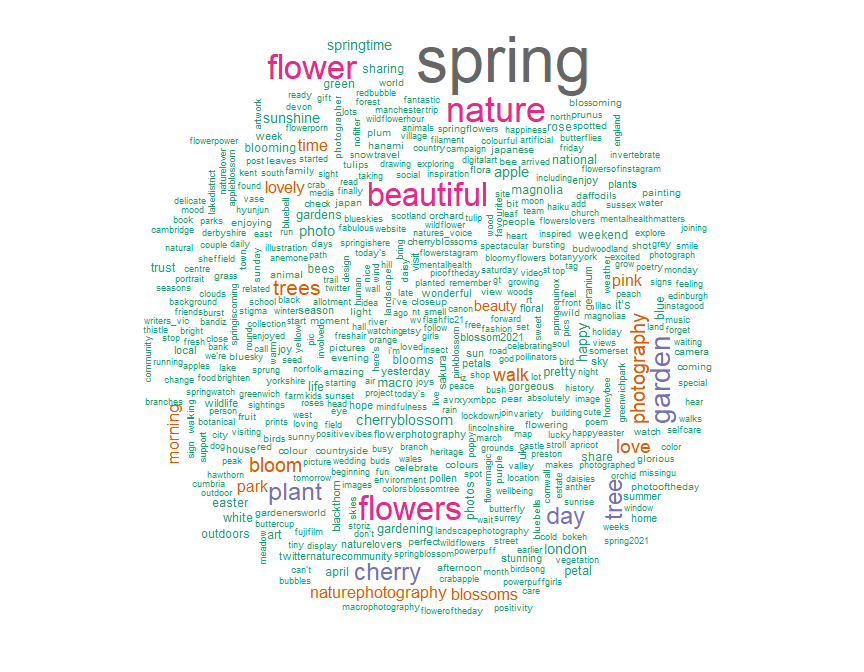
\includegraphics{twitter-blossom-watch-2021_files/figure-latex/count-words-1.pdf}

\hypertarget{who-has-280-characters}{%
\subsection{Who has 280 characters?}\label{who-has-280-characters}}

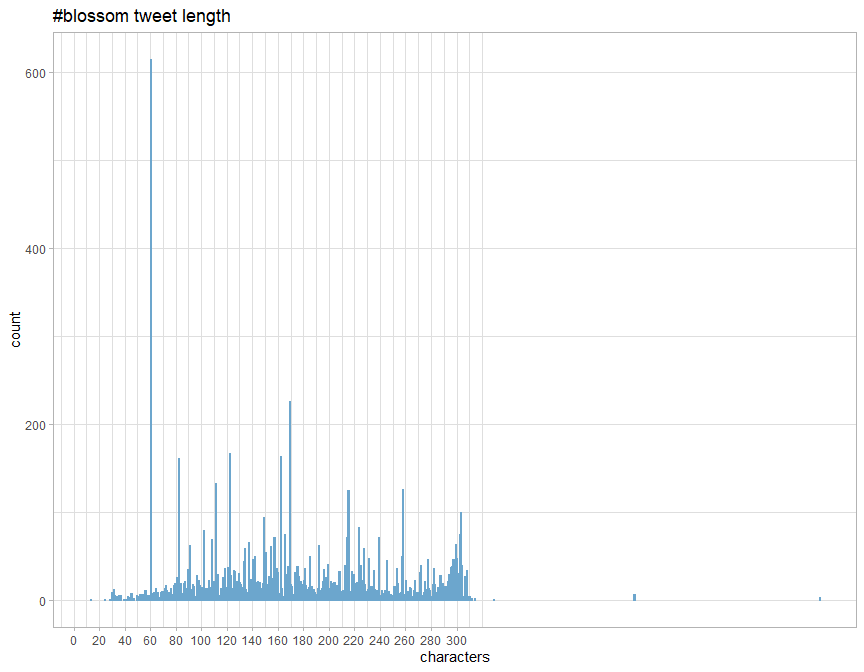
\includegraphics{twitter-blossom-watch-2021_files/figure-latex/count-tweet-length-1.pdf}

\end{document}
